\section{Experiment of learning motion primitives}
\label{cha5:sec3}




This section presents the implementation of the system in learning bi-manual grasping motion primitives. Bi-manual grasping is regularly used in daily life. One of the most commonly used strategies is putting two hands at the opposite sides of a bulky object to apply antipodal grasps (Figure~\ref{fig:graspdemo}). These motion primitives, including an approaching motion and a lifting motion, can be used to grasp many different objects. In our experiment, we focus on learning this strategy and verify that it can be generalized to grasp objects in unseen scenarios.

The strategy is demonstrated in two different scenarios: grasping boxes with different sizes and grasping boxes placed on different heights. As explained in section~\ref{cha5:sec2:demonstration}, the demonstrations are chosen to define the boundary situations of the grasping motions. In this experiment, four different motion primitives are demonstrated: grasping the biggest feasible box,  grasping the smallest feasible box, grasping the lowest feasible box and grasping the highest feasible box. Objects with size or height outside the feasible area might be able to be grasped by the same strategy, but the motion may be very close to infeasible joint angles or is not natural for human behaviour. In our case, the bi-manual grasp of a box longer than the distance between the left and right elbow is very difficult for the iCub; bi-manual grasp of a very small size box is possible but a human would normally use a single hand grasp.

All the demonstrated motion sequences are recorded by Kinect, a skeleton tracking device widely used both in the gaming industry and in academic research~\citep{ren20123d}. It is a marker-less stereo camera which can automatically detect and track human joint configuration. The output data from Kinect is converted to joint angle space.

In this experiment, the grasping motions only involve the arms. The objects are placed in the working space of the human demonstrator so that the human does not need to change their location to grasp the objects. Due to the technical limitation of Kinect, it cannot record the wrist joint and hence wrist is omitted in our current experiment. In total, 8 degrees of freedom are recorded in the human motion: left shoulder (3D), right shoulder (3D), left elbow (1D) and right elbow (1D). When the hands get contact with the objects, the wrist joints will change due to the force applied by the arm. This adds extract uncertainties to the grasping motion, as well as a certain amount of compliance. As a result the box may rotate a certain angle after lifting (Figure~\ref{graspdemo2}).


Each grasping motion is demonstrated five times. In all demonstrations, the starting postures are the starting posture used by Kinect: the $\Psi$ pose that with two arms raising over the head, both palms facing inside.

The raw data is noisy due to the limitation of the motion capture device. To suppress the noise of the motion signal, we used second order low pass filters to smooth the motion outputs and remove high frequency noise caused by vibration of the machinery. Each motion is low-pass filtered by 1Hz, 5Hz and 10Hz and all the filtered results are supplied as the training data for the Mimesis Model. To find out the outcomes of the motions, we implement the motions in a robot simulator Webots with the iCub.

In the symbolization step (Section~\ref{cha5:sec2:symbolization}), the four motion primitives are encoded by four CHMMs. To completely distinguish between four points we need at least a three dimensional space. Hence we construct a three dimensional proto-symbol space by using the MDS with these CHMMs (Figure~\ref{fig:pss}). To generate new grasping motions, we interpolate (Section~\ref{cha5:sec2:interpolation}) the proto-symbol space with different mixing coefficients. New motions are then generated at each of the interpolation points as detailed in the Section~\ref{cha5:sec2:generating}. These generated motions are then performed by the Webots iCub to examine their effects.


All motions are modelled in ten states, determined by five-fold cross validation, and each state is represented by a single Gaussian to maintain simplicity.


\begin{figure}
  \centering
  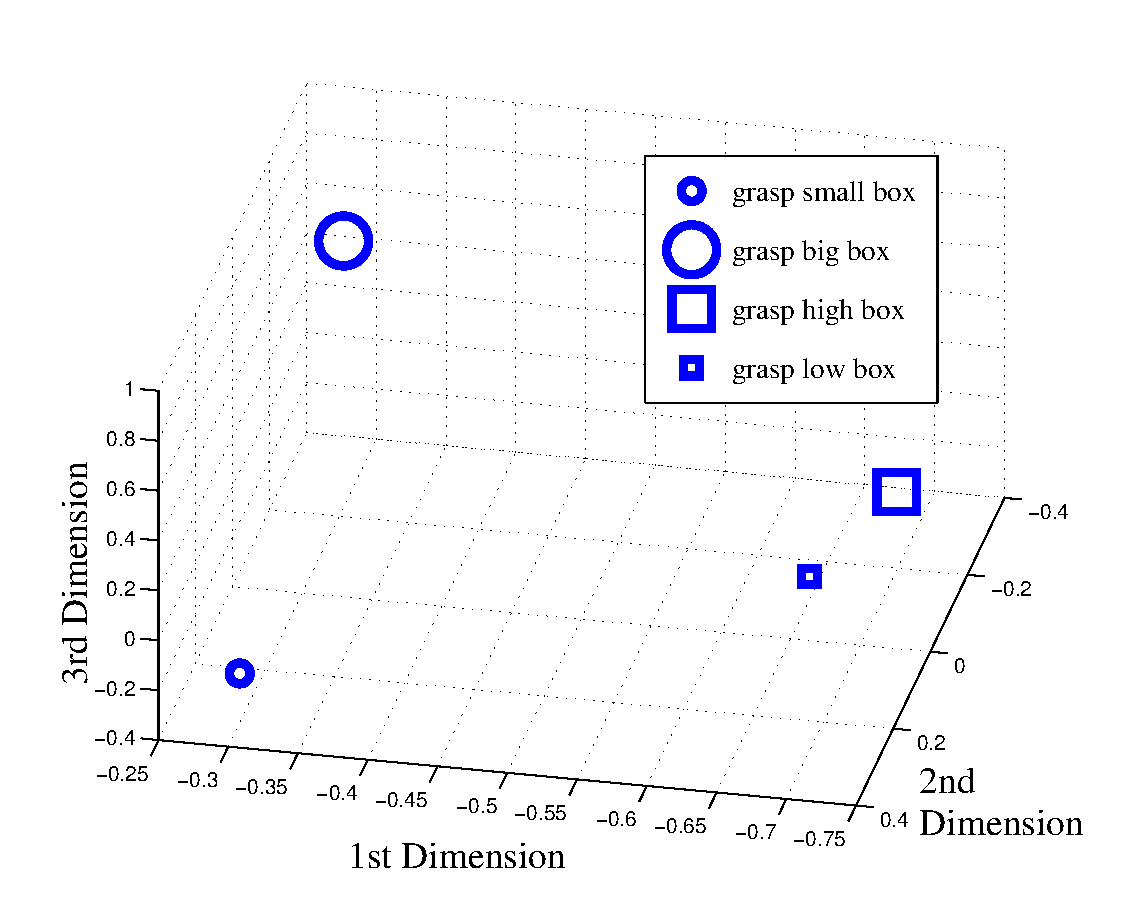
\includegraphics[width=12cm]{./fig_cha5/pss2.eps}
  \caption{ \scriptsize{Proto-symbol space constructed by four motion primitives}
}
    \label{fig:pss}
\end{figure}


\subsection{Grasping different sizes boxes}
\label{cha5:sec3:graspsize}
In this scenario we demonstrate the strategies of grasping different sizes of boxes. The boxes are placed on a cylindrical stand at a height of 84$cm$. The human demonstrator stands 20$cm$ in front of the cylindrical stand (Figure~\ref{fig:graspdemo}).

\begin{figure}
  \centering
  \subfloat[\scriptsize{Motion 1}]{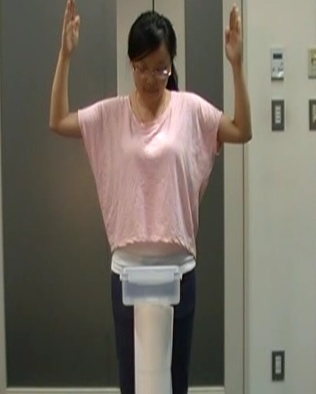
\includegraphics[width=4cm]{./fig_cha5/demosbox1s.jpg}}
  \subfloat[\scriptsize{Motion 2}]{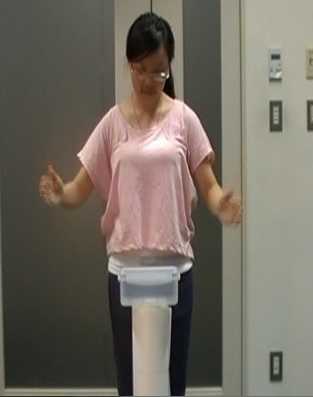
\includegraphics[width=3.96cm]{./fig_cha5/demosbox3s.jpg}}
  \subfloat[\scriptsize{Motion 3}]{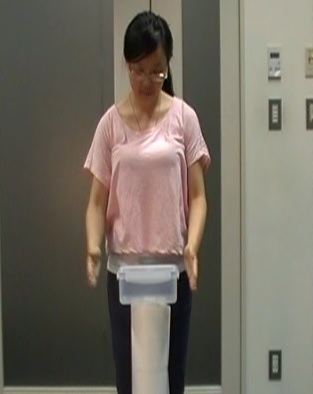
\includegraphics[width=4cm]{./fig_cha5/demosbox4s.jpg}}
  \subfloat[\scriptsize{Motion 4}]{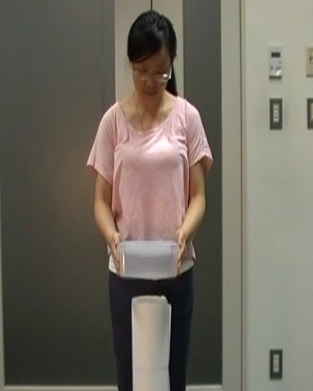
\includegraphics[width=4cm]{./fig_cha5/demosbox6s.jpg}}
  \hspace{1cm}
  \subfloat[\scriptsize{Motion 1}]{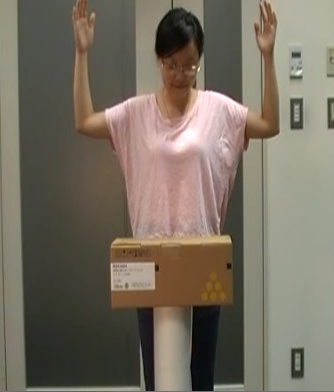
\includegraphics[width=4.2cm]{./fig_cha5/demopinkbox1s.jpg}}
  \subfloat[\scriptsize{Motion 2}]{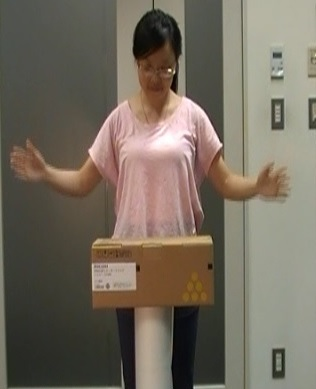
\includegraphics[width=4cm]{./fig_cha5/demopinkbox3s.jpg}}
  \subfloat[\scriptsize{Motion 3}]{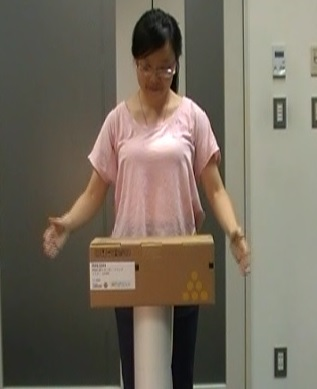
\includegraphics[width=4cm]{./fig_cha5/demopinkbox4s.jpg}}
  \subfloat[\scriptsize{Motion 4}]{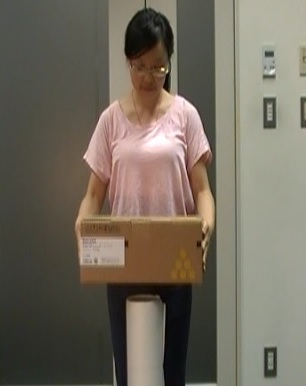
\includegraphics[width=3.9cm]{./fig_cha5/demopinkbox6s.jpg}}
  \caption{ \scriptsize{(a)-(d): Human demonstrating bi-manual grasp of a small box (size 20$cm$(length) $\times$ 15$cm$(width) $\times$ 10$cm$(height)). (e)-(h): Human demonstrating bi-manual grasp of a big box (size 40$cm$(length) $\times$ 20$cm$(width) $\times$ 15$cm$(height))}
}
  \label{fig:graspdemo}
\end{figure}

Figure~\ref{fig:graspdemo} shows the motion sequences. As can be seen from the figure, for grasping the small box, the hands move directly to it, while for grasping the big box, the arms first open to create a certain distance between hands and then close to reduce the distance until contact with the box. This is to avoid unwanted collision with the box during reaching.

New motions are then generated by mixing the demonstrations. To learn the effect of the motions, all demonstrated and generated motions are performed by the robot.
The sizes of the boxes are initially estimated by forward kinematics, and then verified by the robot executing the motion to grasp a box. The motion that can hold a box and lift it vertically without any slipping is considered to be a successful grasp. Table~\ref{trainmixing} shows that the mixing coefficients of the motions and the corresponding size of boxes of successful grasps. Note that mixing coefficients always sum to 1. When we make the mixing coefficient to be 1 for one motion and 0 for the other, the generated motion simply corresponds to the motion with mixing coefficient 1. Linear regression is then applied to find out the correlation between the mixing coefficients and the box sizes.


\begin{table}
\centering
\caption{ \scriptsize{Mixing coefficient of the interpolation points and the box size of successful grasps (training)}}
\renewcommand{\arraystretch}{1.5}
    \begin{tabular}{|>{\centering\arraybackslash}p{8cm}|>{\centering\arraybackslash}p{4cm}|}
    \hline
    Mixing Coefficient of the Interpolation Points & Box size of successful grasps ($cm$)   \\ \hline
    0(small box) 1(big box)   & 43\\ \hline
    0.2(small box) 0.8(big box)   & 39\\ \hline
    0.5(small box) 0.5(big box)   & 35\\ \hline
    0.8(small box) 0.2(big box)   & 28\\ \hline
    1(small box) 0(big box)   & 25\\ \hline
    \end{tabular}
    \label{trainmixing}
\end{table}

\begin{figure}
  \centering
  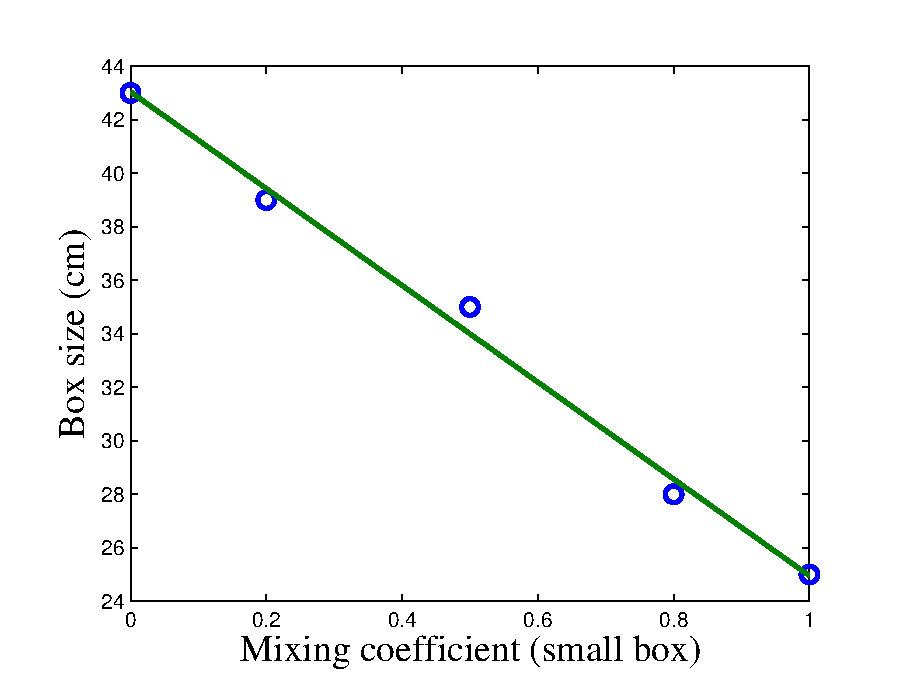
\includegraphics[width=12cm]{./fig_cha5/regression_size.eps}
  \caption{ \scriptsize{Linear regression of the interpolation points}
}
  \label{regression}
\end{figure}


\begin{table}
\centering
\caption{ \scriptsize{Given Box Sizes ($cm$) and the Predicted Mixing Coefficient (testing)}}
\renewcommand{\arraystretch}{1.5}
    \begin{tabular}{|>{\centering\arraybackslash}p{4cm}|>{\centering\arraybackslash}p{8cm}|}
    \hline
    Given Box Size & Predicted Mixing Coefficient \\ \hline
    27    &0.89(small box) 0.11(big box)\\ \hline
    30     &0.72(small box) 0.27(big box)\\ \hline
    36    &0.44(small box) 0.56(big box)\\ \hline
    40     &0.16(small box) 0.74(big box)\\ \hline
    \end{tabular}

    \label{predictmixing}
\end{table}



Figure~\ref{regression} shows the linear regression result of the mixing coefficients and the size of successful grasped boxes. With the regression result, given a size of box, the mixing coefficient of generating a corresponding grasping motion can be deduced. To test this method, we applied this method to grasp four un-demonstrated boxes with different sizes. All of them can be successfully lifted by the synthesis grasping motions. Table~\ref{predictmixing} lists the given boxes size and the computed mixing coefficient and Figure~\ref{graspdemo2} shows the corresponding motions.


\begin{figure}

  \hspace{-1.2cm}
  \begin{minipage}[c]{1\textwidth}
  \subfloat[\scriptsize{Motion 1}]{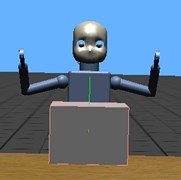
\includegraphics[width=4cm]{./fig_cha5/icub27box1_crop.jpg}}
  \subfloat[\scriptsize{Motion 2}]{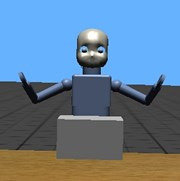
\includegraphics[width=3.96cm]{./fig_cha5/icub27box2_crop.jpg}}
  \subfloat[\scriptsize{Motion 3}]{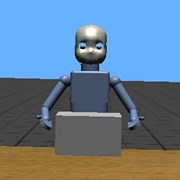
\includegraphics[width=4cm]{./fig_cha5/icub27box3_crop.jpg}}
  \subfloat[\scriptsize{Motion 4}]{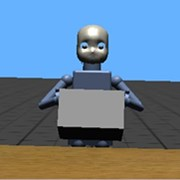
\includegraphics[width=4cm]{./fig_cha5/icub27box4_crop.jpg}}
  \end{minipage}

  \hspace{-1.2cm}
  \begin{minipage}[c]{1\textwidth}
  \subfloat[\scriptsize{Motion 1}]{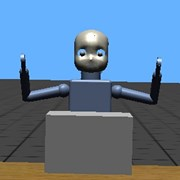
\includegraphics[width=4cm]{./fig_cha5/icub30box1_crop.jpg}}
  \subfloat[\scriptsize{Motion 2}]{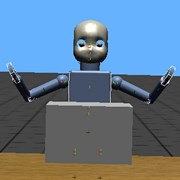
\includegraphics[width=4cm]{./fig_cha5/icub30box2_crop.jpg}}
  \subfloat[\scriptsize{Motion 3}]{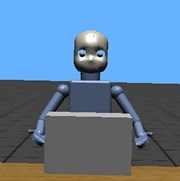
\includegraphics[width=4cm]{./fig_cha5/icub30box3_crop.jpg}}
  \subfloat[\scriptsize{Motion 4}]{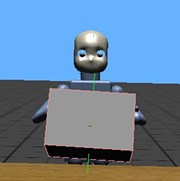
\includegraphics[width=4cm]{./fig_cha5/icub30box4_crop.jpg}}
  \end{minipage}

  \hspace{-1.2cm}
  \begin{minipage}[c]{1\textwidth}
  \subfloat[\scriptsize{Motion 1}]{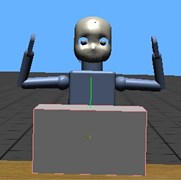
\includegraphics[width=4cm]{./fig_cha5/icub35box1_crop.jpg}}
  \subfloat[\scriptsize{Motion 2}]{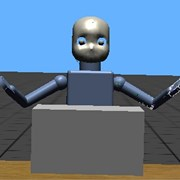
\includegraphics[width=4cm]{./fig_cha5/icub35box2_crop.jpg}}
  \subfloat[\scriptsize{Motion 3}]{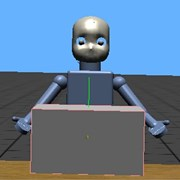
\includegraphics[width=4cm]{./fig_cha5/icub35box3_crop.jpg}}
  \subfloat[\scriptsize{Motion 4}]{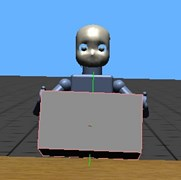
\includegraphics[width=4cm]{./fig_cha5/icub35box4_crop.jpg}}
  \end{minipage}

  \hspace{-1.2cm}
  \begin{minipage}[c]{1\textwidth}
  \subfloat[\scriptsize{Motion 1}]{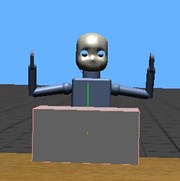
\includegraphics[width=4cm]{./fig_cha5/icub40box1_crop.jpg}}
  \subfloat[\scriptsize{Motion 2}]{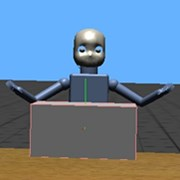
\includegraphics[width=4cm]{./fig_cha5/icub40box2_crop.jpg}}
  \subfloat[\scriptsize{Motion 3}]{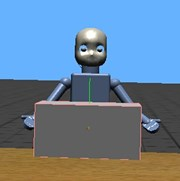
\includegraphics[width=4cm]{./fig_cha5/icub40box3_crop.jpg}}
  \subfloat[\scriptsize{Motion 4}]{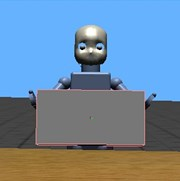
\includegraphics[width=4cm]{./fig_cha5/icub40box4_crop.jpg}}
  \end{minipage}


    \vspace{-0.5cm}
    \caption{ \scriptsize{Robot grasping different boxes with the generated motions.
  (a)-(d) Box size 27$cm$. (e)-(h) Box size 30$cm$. (i)-(l) Box size 35$cm$. (m)-(p) Box size 40$cm$.}}
    \label{graspdemo2}
\end{figure}

\subsection{Grasping boxes from different positions}
\label{sbsec:diffheight}
In this scenario the goal is to grasp boxes from different heights. Two motions are demonstrated to grasp a high and a low box. In the demonstrations the high box is placed at the height of $150 cm$ and the low box is placed at $70 cm$. In this case, the two demonstrations are not only different in the arm trajectories but also different in the time duration (Figure~\ref{highlowjoint}). The motion of grasping the high box takes less time than grasping the low box as the initial hand position is closer to the box position. At the same time the lifting parts of the motions are different: for the high box the lifting distance is smaller than the low box because of the joint limits of the arms.

\begin{figure}
    \centering
    \subfloat[\scriptsize{Grasping box in a low position}]{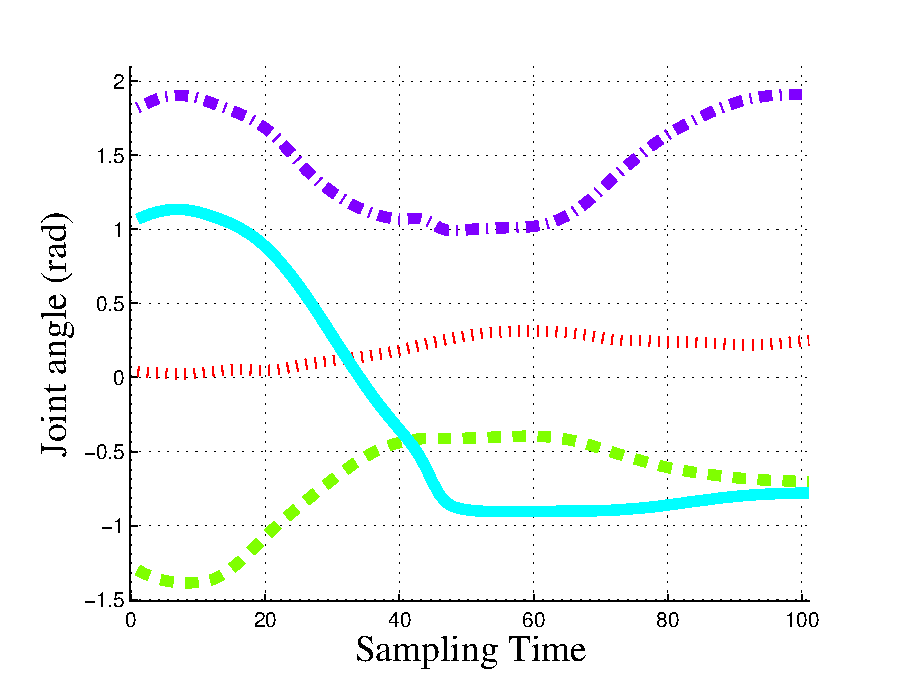
\includegraphics[width=8cm]{./fig_cha5/joint_sbox_adj.eps}}
    \subfloat[\scriptsize{Grasping box in a high position}]{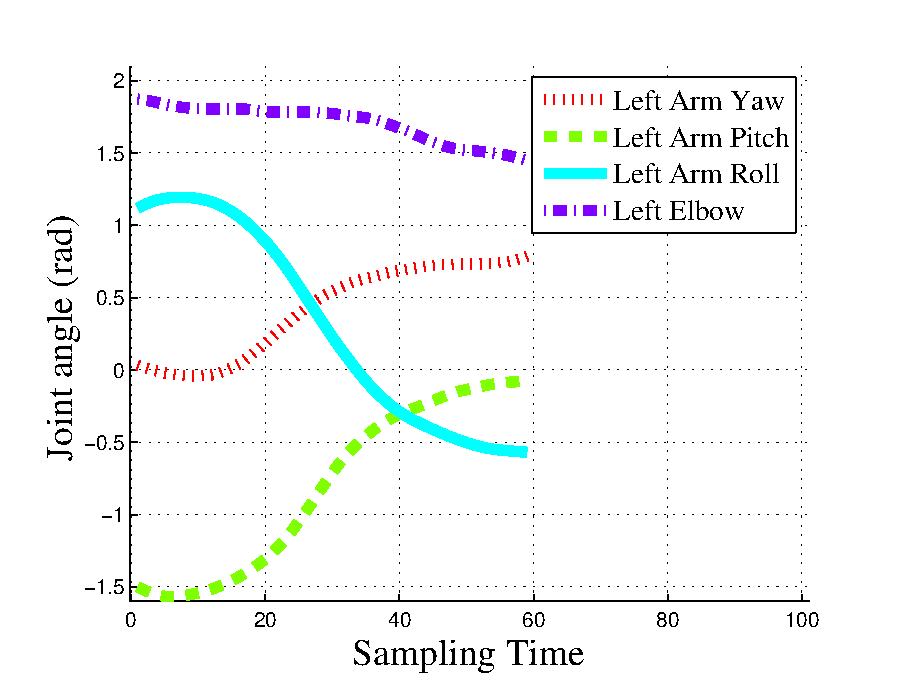
\includegraphics[width=8cm]{./fig_cha5/joint_ssbox_high356.eps}}
    \caption{ \scriptsize{(a) Left arm motion of a human demonstration of grasping a low box. (b) Left arm motion of a human demonstration of grasping a high box.}}
\label{highlowjoint}
\end{figure}
Following the same process as described above, we interpolate between the motions for grasping the low box and the high box (Table~\ref{trainhigh}). We apply linear regression and hence find out the correlation between the mixing coefficients and the heights of the box (Figure~\ref{highregression}).

With the learned correlation, we query the mixing coefficients for four different un-demonstrated heights (Table~\ref{predictmixing_high}). The generated motions are tested with the Webots iCub, which successfully lifted all the boxes. %Besides the height of the box, the time of performing the task and the lifting distances are also interpolated .

\begin{table}
\centering
\renewcommand{\arraystretch}{1.5}
    \begin{tabular}{|>{\centering\arraybackslash}p{8cm}|>{\centering\arraybackslash}p{4cm}|}
    \hline
    Mixing Coefficient &  Box height($cm$)  \\ \hline
    0(high box) 1(low box)   & 49\\ \hline
    0.2(high box) 0.8(low box)   & 53\\ \hline
    0.5(high box) 0.5(low box)   & 58\\ \hline
    0.8(high box) 0.2(low box)   & 62\\ \hline
    1(high box) 0(low box)   & 64\\ \hline
    \end{tabular}
    \caption{\scriptsize{Mixing coefficient of the interpolation points and the box heights (center of mass from the ground) of successful grasps (training).}}
    \vspace{-0.5cm}
    \label{trainhigh}
\end{table}

\begin{figure}
  \centering
  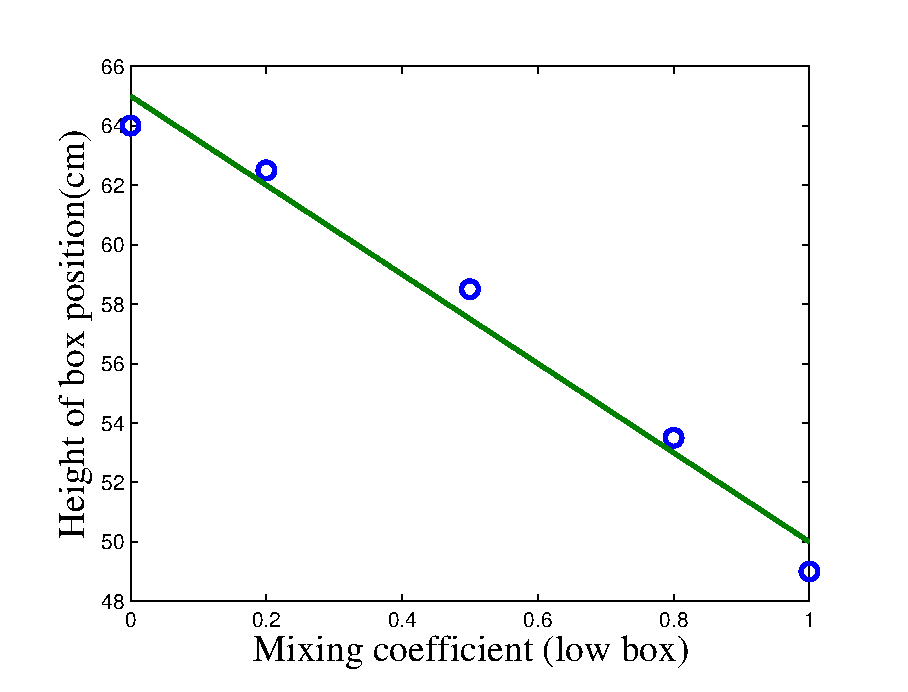
\includegraphics[width=12cm]{./fig_cha5/regression_high.eps}
  \caption{ \scriptsize{Linear regression of the interpolation points}
}
    \vspace{-0.5cm}
    \label{highregression}
\end{figure}

\begin{table}
\centering
\renewcommand{\arraystretch}{1.5}
    \begin{tabular}{|>{\centering\arraybackslash}p{4cm}|>{\centering\arraybackslash}p{8cm}|}
    \hline
    Given Box Height & Predicted Mixing Coefficient \\ \hline
    50    &0.02(high box) 0.98(low box)\\ \hline
    55     &0.34(high box) 0.66(low box)\\ \hline
    60    &0.66(high box) 0.34(low box)\\ \hline
    63     &0.86(high box) 0.14(low box)\\ \hline
    \end{tabular}
    \caption{\scriptsize{Given Box Height ($cm$) and the Predicted Mixing Coefficient (testing)}}
    \label{predictmixing_high}
\end{table}

\begin{figure*}
  \centering
  \hspace{-2.2cm}
  \begin{minipage}[c]{1\textwidth}
  \subfloat[\scriptsize{Motion 1}]{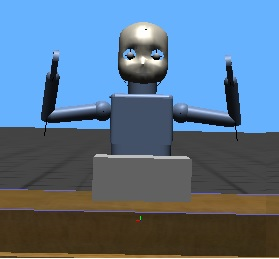
\includegraphics[width=4cm]{./fig_cha5/sbox_high356_ssbox_adj_005_095_1.jpg}}
  \subfloat[\scriptsize{Motion 2}]{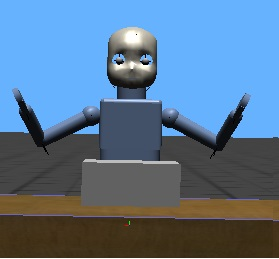
\includegraphics[width=4cm]{./fig_cha5/sbox_high356_ssbox_adj_005_095_2.jpg}}
  \subfloat[\scriptsize{Motion 3}]{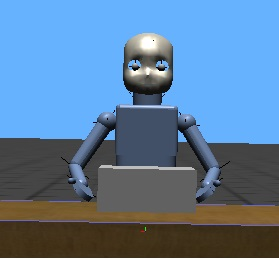
\includegraphics[width=4cm]{./fig_cha5/sbox_high356_ssbox_adj_005_095_3.jpg}}
  \subfloat[\scriptsize{Motion 4}]{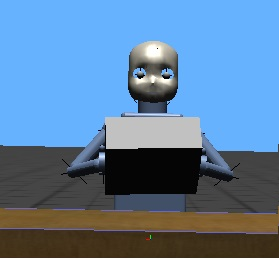
\includegraphics[width=4cm]{./fig_cha5/sbox_high356_ssbox_adj_005_095_4.jpg}}
  \end{minipage}

  \hspace{-2.2cm}
  \begin{minipage}[c]{1\textwidth}
  \subfloat[\scriptsize{Motion 1}]{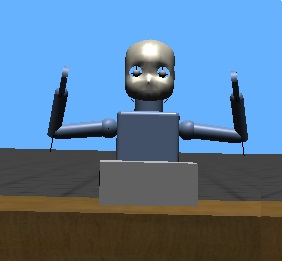
\includegraphics[width=4cm]{./fig_cha5/sbox_high356_ssbox_adj_167_833_1.jpg}}
  \subfloat[\scriptsize{Motion 2}]{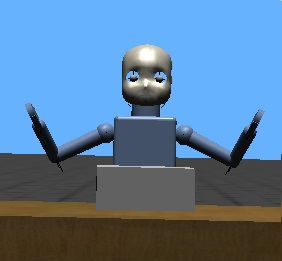
\includegraphics[width=4cm]{./fig_cha5/sbox_high356_ssbox_adj_167_833_2.jpg}}
  \subfloat[\scriptsize{Motion 3}]{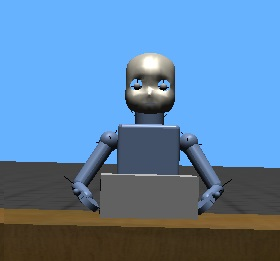
\includegraphics[width=4cm]{./fig_cha5/sbox_high356_ssbox_adj_167_833_3.jpg}}
  \subfloat[\scriptsize{Motion 4}]{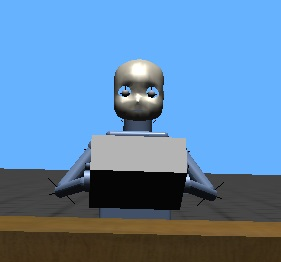
\includegraphics[width=4cm]{./fig_cha5/sbox_high356_ssbox_adj_167_833_4.jpg}}
  \end{minipage}

  \hspace{-2.2cm}
  \begin{minipage}[c]{1\textwidth}
  \subfloat[\scriptsize{Motion 1}]{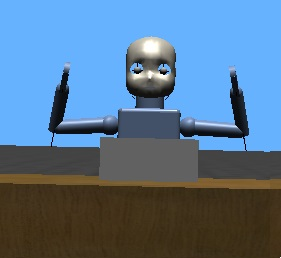
\includegraphics[width=4cm]{./fig_cha5/sbox_high356_ssbox_adj_433_567_1.jpg}}
  \subfloat[\scriptsize{Motion 2}]{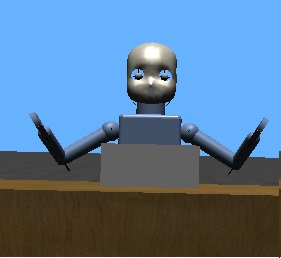
\includegraphics[width=4cm]{./fig_cha5/sbox_high356_ssbox_adj_433_567_2.jpg}}
  \subfloat[\scriptsize{Motion 3}]{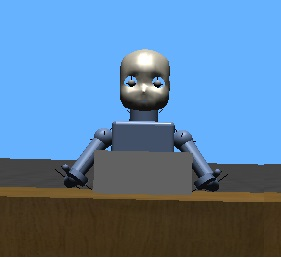
\includegraphics[width=4cm]{./fig_cha5/sbox_high356_ssbox_adj_433_567_3.jpg}}
  \subfloat[\scriptsize{Motion 4}]{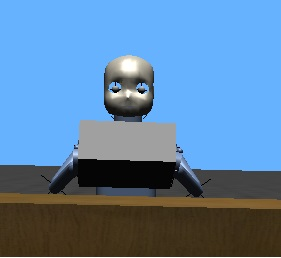
\includegraphics[width=4cm]{./fig_cha5/sbox_high356_ssbox_adj_433_567_4.jpg}}
  \end{minipage}

  \hspace{-2.2cm}
  \begin{minipage}[c]{1\textwidth}
  \subfloat[\scriptsize{Motion 1}]{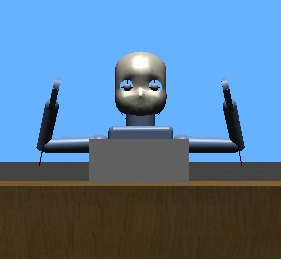
\includegraphics[width=4cm]{./fig_cha5/sbox_high356_ssbox_adj_667_333_1.jpg}}
  \subfloat[\scriptsize{Motion 2}]{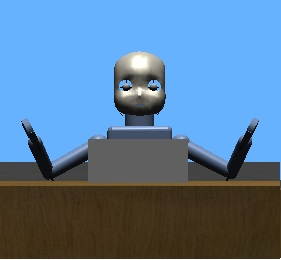
\includegraphics[width=4cm]{./fig_cha5/sbox_high356_ssbox_adj_667_333_2.jpg}}
  \subfloat[\scriptsize{Motion 3}]{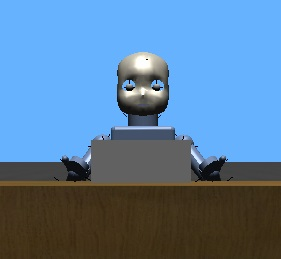
\includegraphics[width=4.02cm]{./fig_cha5/sbox_high356_ssbox_adj_667_333_3.jpg}}
  \subfloat[\scriptsize{Motion 4}]{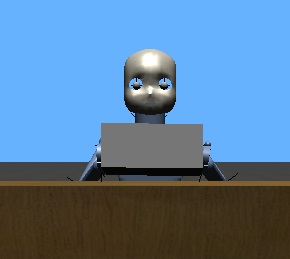
\includegraphics[width=4.1cm]{./fig_cha5/sbox_high356_ssbox_adj_667_333_4.jpg}}
  \end{minipage}

  \caption{ \scriptsize{Robot grasping boxes from different heights with the generated motions.
  (a)-(d) Box at height 50$cm$. (e)-(h) Box at height 55$cm$. (i)-(l) Box at height 60$cm$. (m)-(p) Box at height 63$cm$.}
}
    \label{graspdemo2}
\end{figure*} 